Titanix(Titanic-nix)是一个使用Rust编写的基于Risc-V架构的类Unix操作系统,以异步无栈协程架构为基础,支持多核多任务。目前初赛的所有测试用例已经满分通过,下图是我们队伍(Titanix)的初赛测试通过情况:
\begin{figure}[hbt]
    \centering
    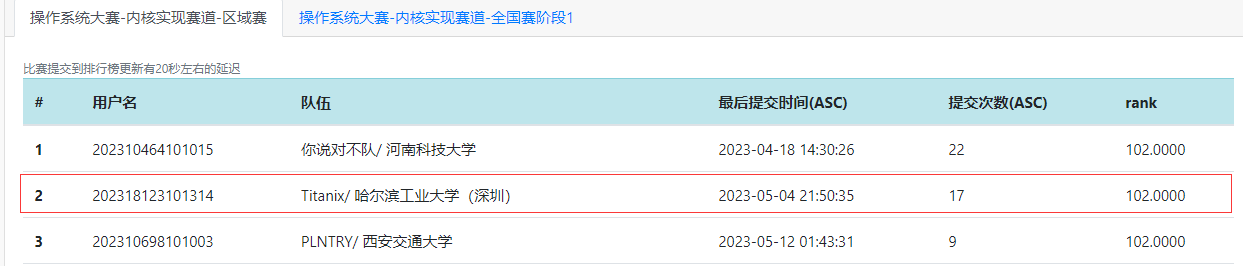
\includegraphics[width=\linewidth]{figure/pre_rank.png}
\end{figure}

此外,Titanix能支持部分libc测试用例以及busybox的部分功能,如sh、ls、echo等,以下是我们各模块的完成情况:

\begin{table}[hbt]
    \caption{Titanix的模块完成情况}
    \centering
    \setlength{\tabcolsep}{10mm}{
    \begin{tabular}{ll}
        \toprule[1.5pt]
        模块 & 完成情况 \\
        \midrule[1pt]
            进程管理   & \makecell[l]{实现分时多任务无栈异步协程调度;\\ 实现多线程运行与回收; \\ 实现多核并行; }      \\
        \midrule[1pt]
            内存管理   & \makecell[l]{实现虚拟内存,用户和内核共享地址空间;\\ 实现页缓存和块缓存,减少IO次数; \\ 实现文件映射和匿名映射;\\ 实现懒分配与写时复制; }     \\
        \midrule[1pt]
            文件系统   & \makecell[l]{实现虚拟文件系统,支持FAT32文件系统接入; \\ 实现Inode缓存,减少IO次数; \\ 利用hash加速Inode查找; \\ TODO}     \\
        \midrule[1pt]
            信号系统   & TODO     \\
        \midrule[1pt]
            多核支持   & TODO     \\
        \bottomrule[1.5pt]
    \end{tabular}
    }
\end{table}

